\mychapter{Metodologia}
\label{Métodos de implementação}
\paragraph{
Finalizada uma primeira perspectiva na primeira parte do projeto, primeiramente foi decidido um planejamento de como deveria ser o percorrer do projeto ao longo do período de desenvolvimento do trabalho.\\
O primeiro trabalho a ser feito, com uma maior prioridade, claramente era a compra, uma vez que tal tarefa era um trabalho cujo tempo de resposta (entrega, no caso) era totalmente indendente dos esforços dos componentes do time. Por essaa razão, nessa primeira tarefa, os integrantes focaram-se em aprender a usar os componentes comprados, projetar onde e como os componentes seriam utilizados.
Feito o pedido de compras, o segundo passo foi a implementação da parte do sistema que envolvia o software estudado. Para a implementação do software, o grupo utilizou de conhecimentos adquiridos nos períodos de estágio e nas aulas para se organizar e implementar o software o mais rápido possível para que uma maior atenção pudesse ser dada ao hardware, uma vez que esse era a parte do projeto cujo conhecimento era mais reduzido. Para tanto, o sistema utilizado foi: a repartição do software em histórias, e o registro dessas repartições em um organizador (no caso, o aplicativo de gerenciamento de tarefas Trello). Durante o período de estágio, como as possíbilidades de encontros dos membros era menor, as tarefas eram então distribuídas aos membro e uma vez por semana, normalmente no sábado, era realizada um pequeno encontro para discutir o que foi feito, juntar as partes e decidir as próximas tarefas a serem feita, sendo que o prazo que o grupo escolheu para o software, foi de até o final do período de estágio (final de agosto de 2015) o componente de software estivesse terminado e testado, ou, na pior das hipóteses, terminado.
}

\begin{figure}
\centering
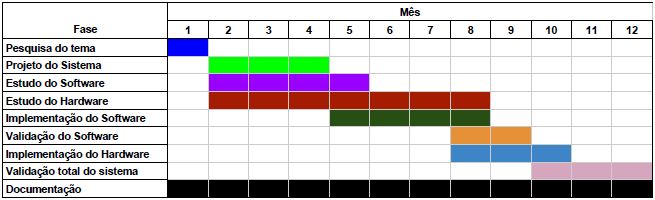
\includegraphics[width=1\textwidth]{figuras/cronogram.png}
\caption{\label{fig:cronogram} Cronograma geral do projeto}
\end{figure}